\chapter{Presupuesto y planificación temporal}
\label{cap: planificacion_presupuesto}

En este capítulo se detalla la planificación adoptada en el transcurso de este proyecto. Se ha trabajado con dos líneas de planificación coordinadas: una línea de planificación estratégica enfocada en la definición de los paquetes de trabajo y los plazos generales de ejecución, y una línea de planificación ágil enfocada en realizar un seguimiento más específico de cada pequeña tarea para valorar su estado. También se tratarán aspectos económicos y el presupuesto manejado para la consecución de este trabajo en forma de costes.

\section{Planificación estratégica}
Para la definición del proyecto en unidades funcionales más pequeñas se ha optado por emplear un modelo \acrshort{EDP}. La \acrshort{EDP} definida para este proyecto cuenta con varias fases con  su propio marco temporal definido en el diagrama Gantt. Estas fases son:

\begin{enumerate}
    \item \textbf{Estudio previo:} Comprensión del flujo de trabajo seguido en sistemas de  fabricación \acrshort{AM} y estado actual del problema.
    \item \textbf{Diseño de arquitectura:} Etapa de diseño de modelo de comunicaciones y flujo de trabajo a implementar en la estación robotizada.
    \item \textbf{Ecosistema ROS2:} Fase de configuración de un entorno o ecosistema informático común a todo el marco de proyecto con los programas y elementos informáticos necesarios para ello.
    \item \textbf{Adquisición de datos:} Diseño de un sistema de adquisición de datos directa desde el UR y con capacidad de gestionarse desde la unidad de operación.
    \item \textbf{Trazado de trayectorias:} Sistema de lectura de archivos de trayectorias de impresión y movimiento automático del manipulador robótico.
    \item \textbf{Control de temperatura:} Control de temperatura de la cama de impresión comandado desde la unidad central de la estación de fabricación.
    \item \textbf{Integración:} Implementación de todos los sistemas desarrollados en un único elemento funcional.
    \item \textbf{Documentación:} Redacción de manual de uso del sistema, subida del proyecto al repositorio y redacción de la memoria.
\end{enumerate}


\begin{landscape}
    \subsection{Estructura de descomposicón del proyecto}
    La Figura \ref{fig:edp_completa} muestra la \acrfull{EDP}. En ella se indica un desglose de aquellas tareas de mayor relevancia dentro de este trabajo y cómo se han organizado en paquetes temáticos y/o funcionales. Aquellos paquetes de trabajo que impliquen el desarrollo de alguna tecnología cuentan con una sección inferior enfocada en la validación de su correcto funcionamiento.
        \begin{figure}[h!]
            \centering
            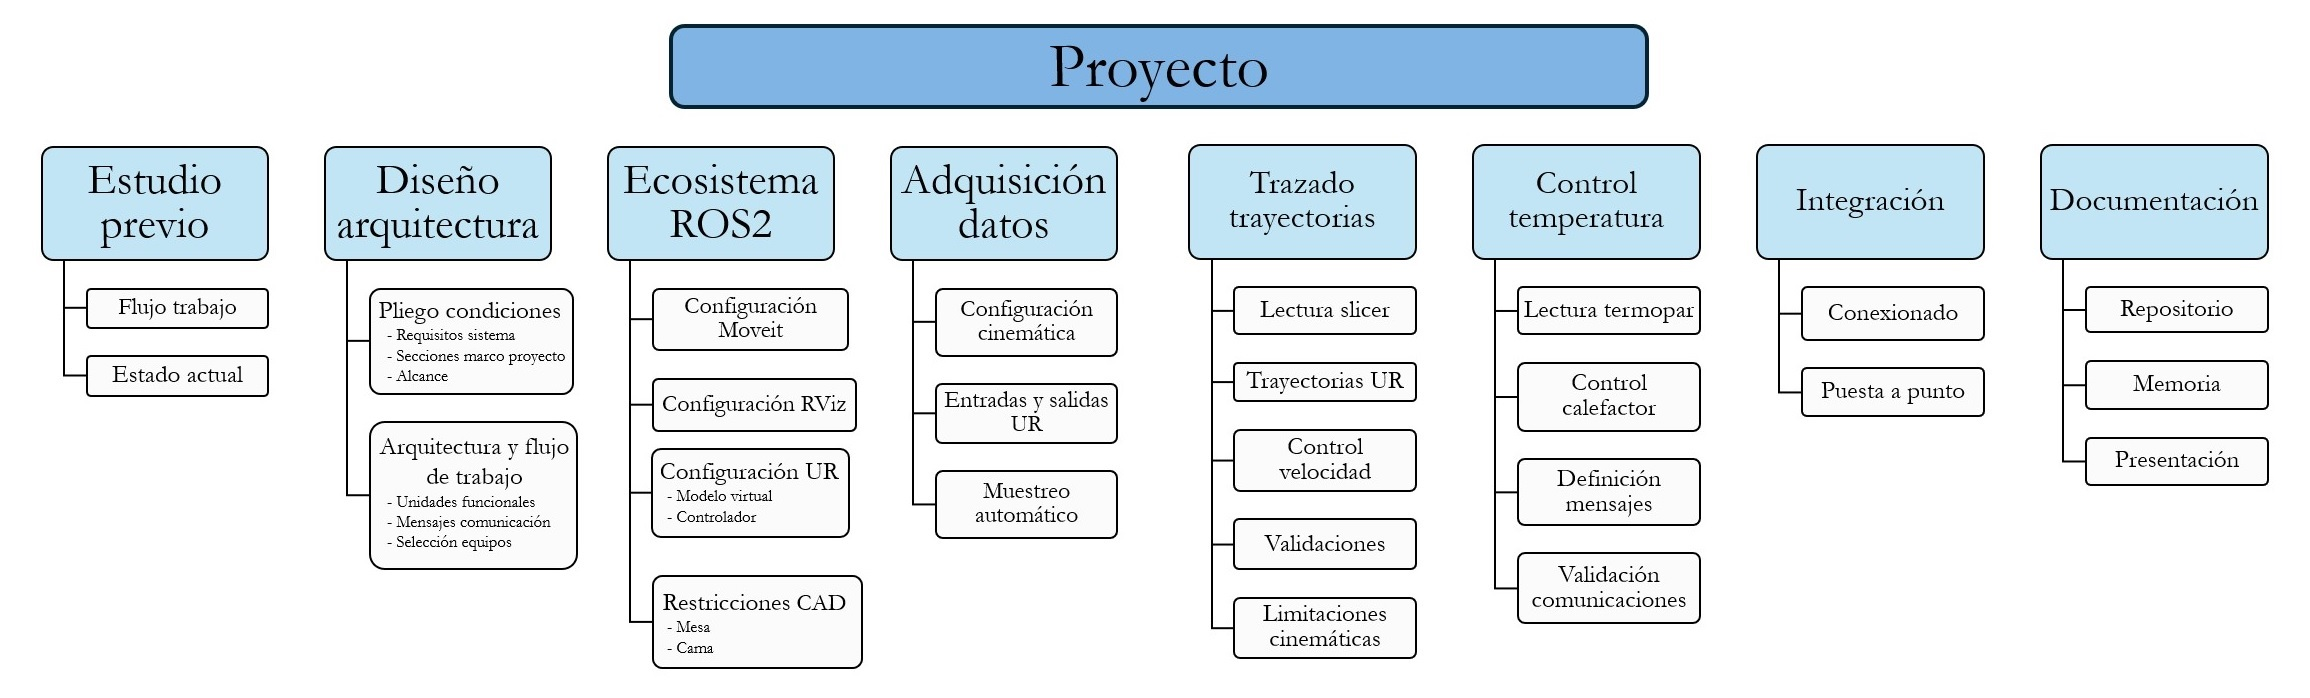
\includegraphics[width=\linewidth, height=8cm]{figuras/edp_completa_horizontal.jpg}
            \caption{Estructura de descomposición del proyecto}
            \label{fig:edp_completa}
        \end{figure}
\end{landscape}
\restoregeometry

\newpage
\begin{landscape}
    \subsection{Diagrama de Gant}
    La Figura \ref{fig:gantt} muestra el diagrama de Gantt utilizado en este proyecto para gestionar de forma clara las diferentes tareas y subdivisiones en el tiempo. Es importante destacar que cada vez que se finalizaba el desarrollo de un paquete de trabajo relacionado con la implementación de una tecnología, se opta por sucederle de una etapa de validación de su correcto funcionamiento.
        \begin{figure}[h!]
            \centering
            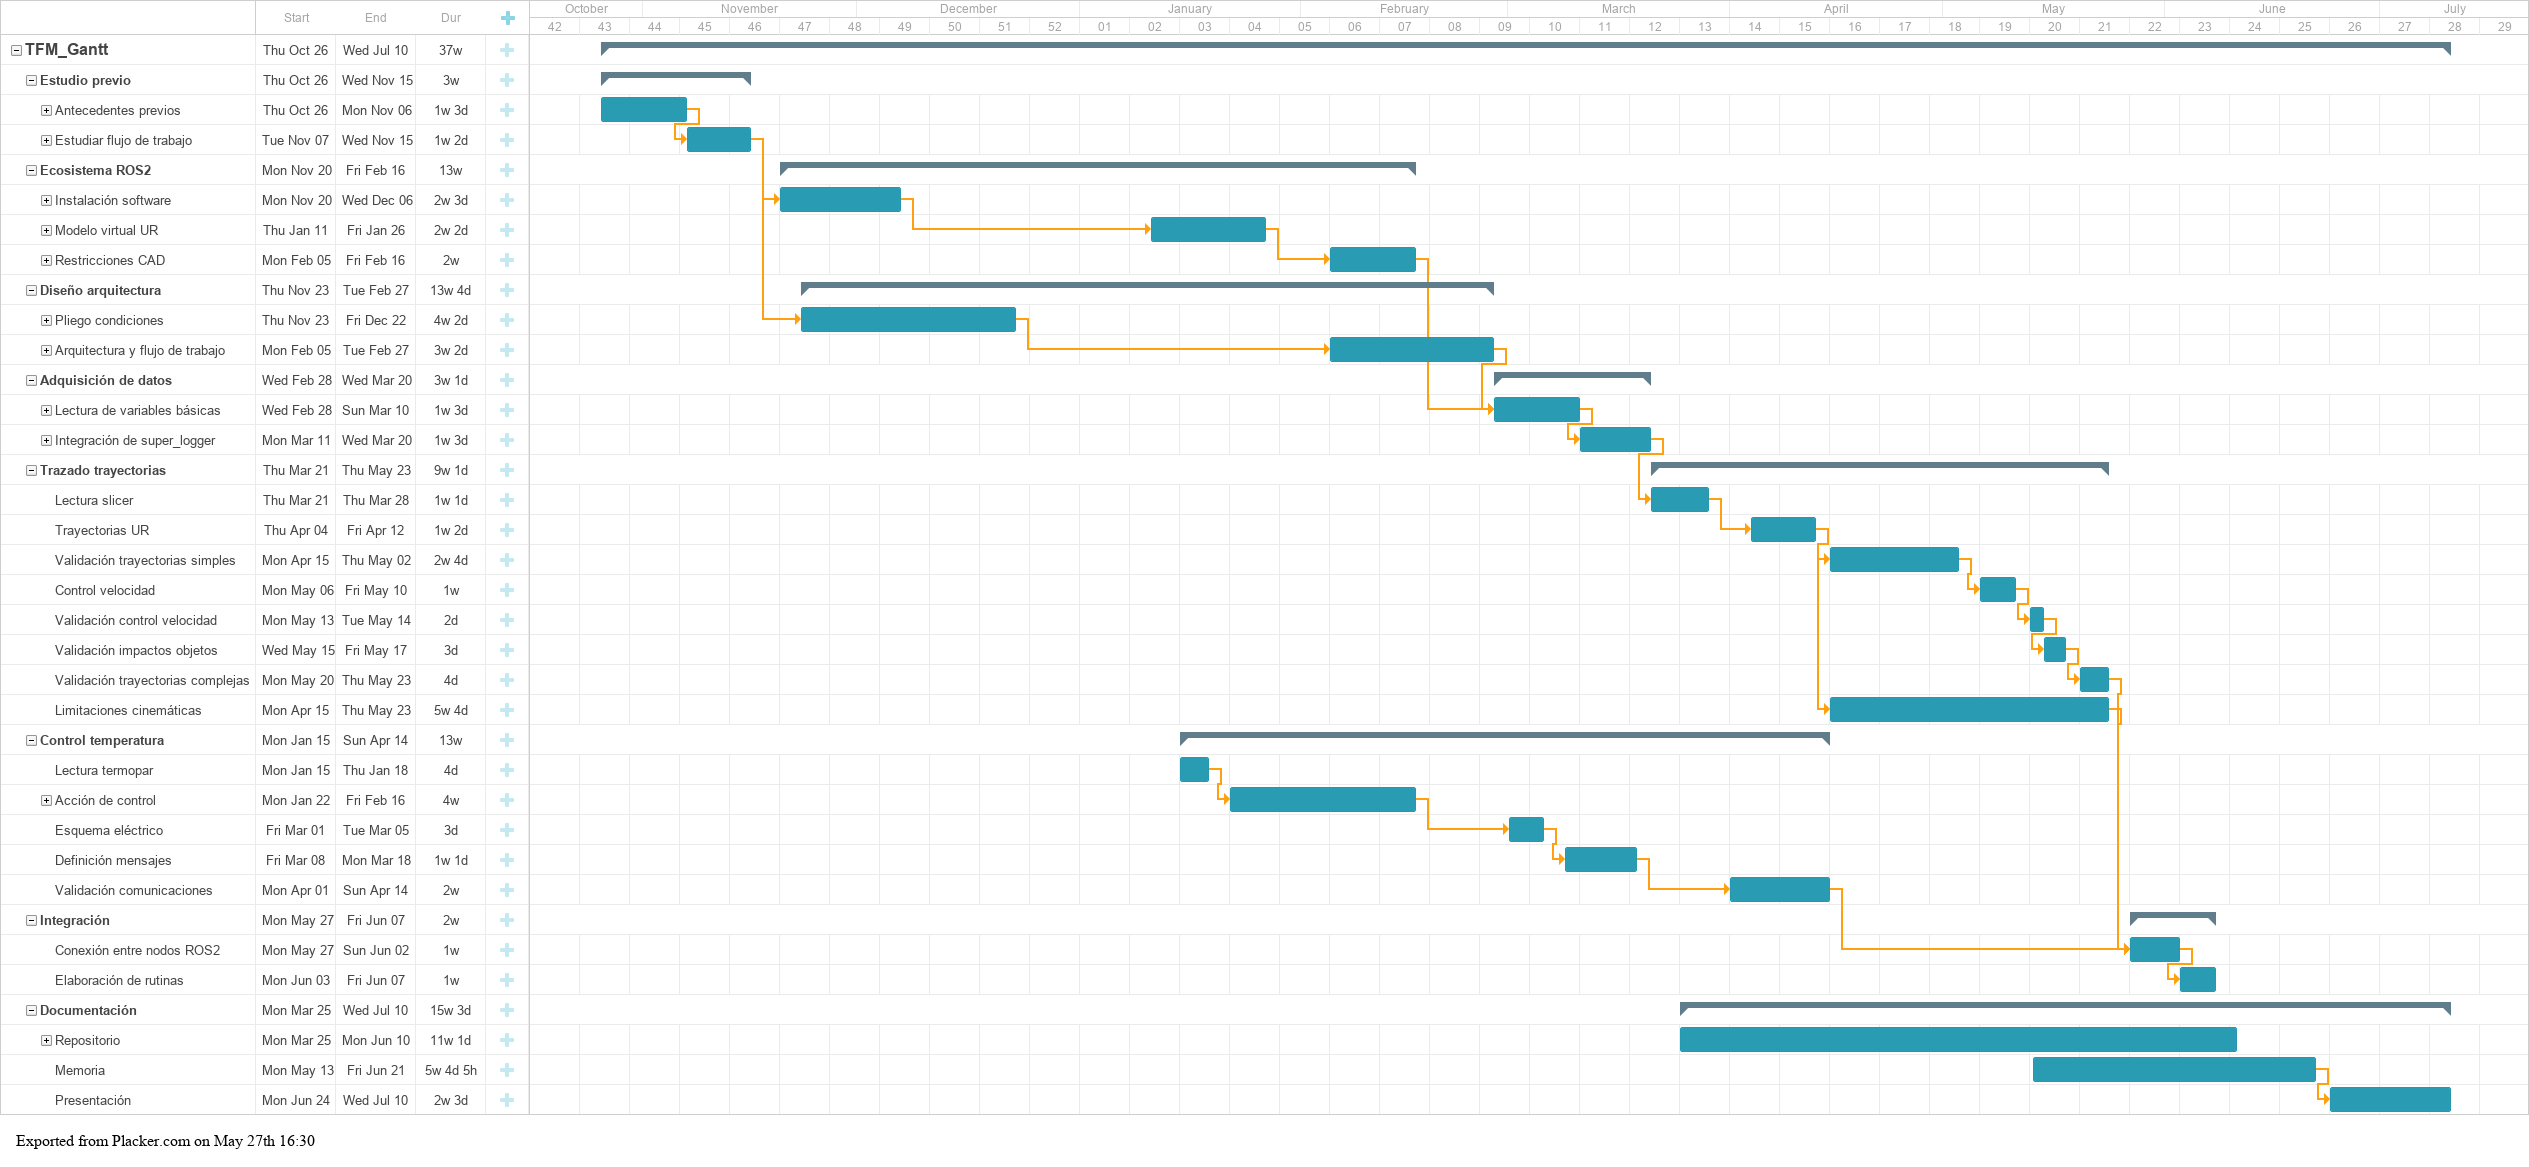
\includegraphics[width=\linewidth]{figuras/gantt_horizontal.png}
            \caption{Diagrama Gantt del proyecto}
            \label{fig:gantt}
        \end{figure}
\end{landscape}
\restoregeometry
\newpage

\section{Planificación ágil}
Para tener un seguimiento continuado de las tareas generales del proyecto, se opta por dividir el trabajo en tareas más pequeñas que pueden evaluarse y modificar rápidamente. Esta línea utiliza la metodología Kanban, que es una técnica ágil para gestionar el trabajo con un enfoque en la mejora continua y la eficiencia.  De este modo se puede definir claramente el flujo de trabajo en cada tarea, valorando su estado y la prioridad de ejecución. Otra ventaja de la implementación de este tipo de planificación en estructuras más pequeñas es la capacidad de respuesta ágil sin necesidad de modificar las líneas generales del proyecto.

La Figura \ref{fig:kanban_TFM} muestra un ejemplo del tablero Kanban seguido durante la ejecución de este proyecto. La Figura \ref{fig:sprints_kanban_TFM} muestra algunos de los \textit{sprints} o entregables que el autor del proyecto se pone como límite de tiempo para cada conjunto subtareas. Estas figuras son ilustrativas y no tienen porqué corresponderse con la ejecución real del proyecto.

\begin{figure}[h!]
    \centering
    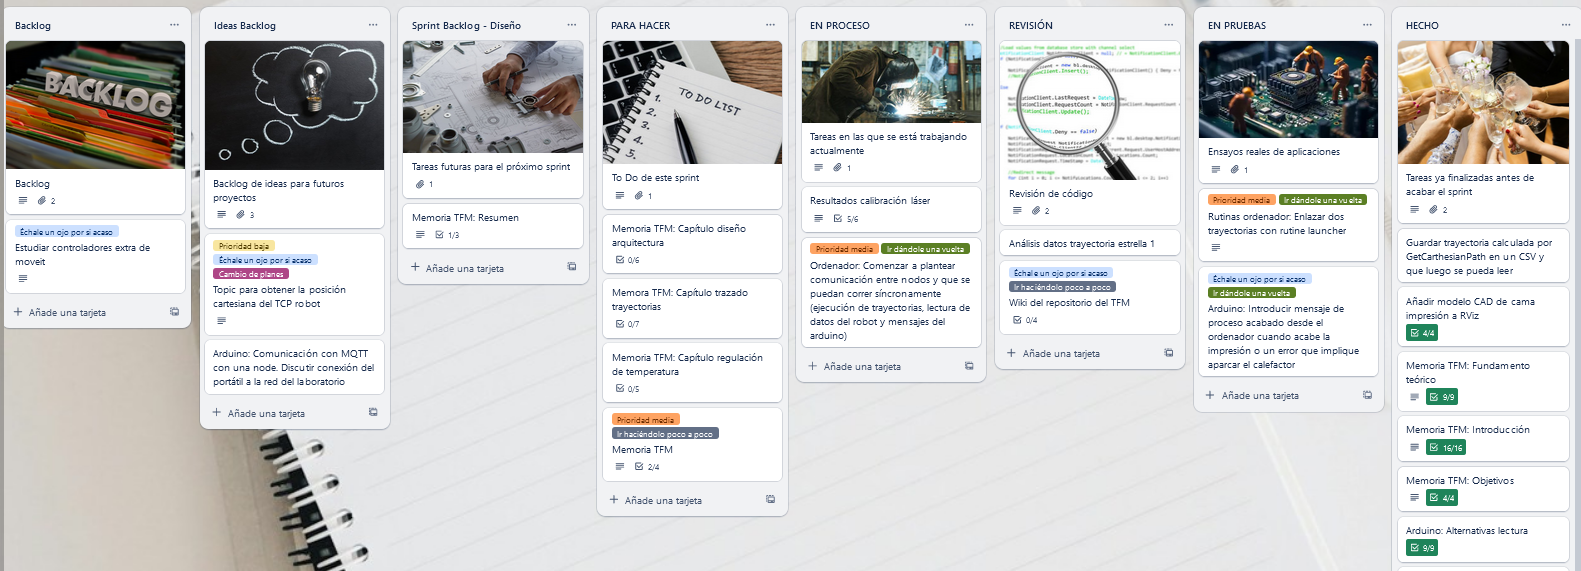
\includegraphics[width=\linewidth]{figuras/tablero_kanban_trello_tfm.png}
    \caption{Tablero Kanban empleado en este proyecto}
    \label{fig:kanban_TFM}
\end{figure}

\begin{figure}[h!]
    \centering
    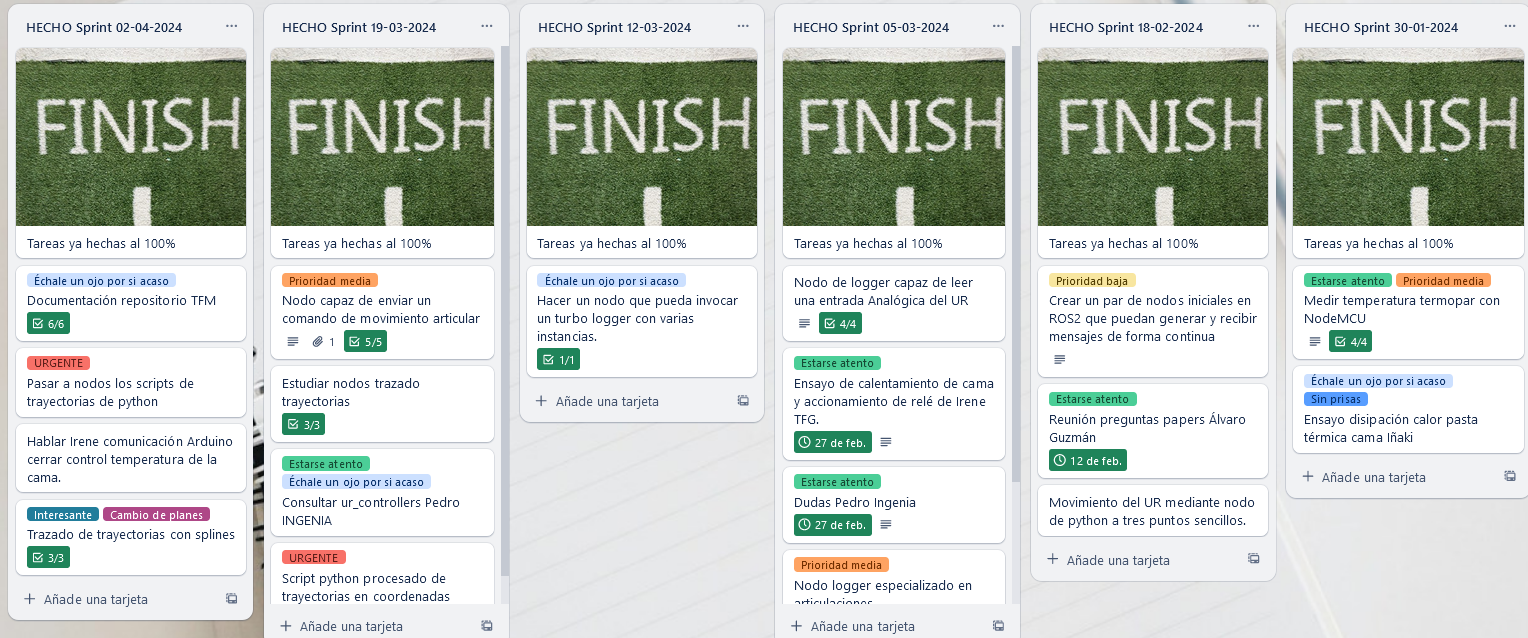
\includegraphics[width=\linewidth]{figuras/tablero_kanban_algunos_sprints.png}
    \caption{Algunos de los sprints de este proyecto}
    \label{fig:sprints_kanban_TFM}
\end{figure}


\section{Presupuesto}

En las siguientes líneas se desglosa el presupuesto del proyecto. El coste total toma en cuenta los costes de adquisición de materiales necesarios, la amortización de los materiales empleados y las labores de coordinación entre el ingeniero director del proyecto (en este caso el tutor) y el ingeniero consultor (el alumno). 

La Tabla \ref{tab:coste_consultor} muestra desglosado el salario del ingeniero consultor en \euro/año y posteriormente se pasa a \euro/h. Se supone una prima de coste social del consultor del 35\% y una tasa de beneficio sobre el proyecto del 20\%. Para la conversión a horas de trabajo se asume un promedio de 1700 h/año.



% Please add the following required packages to your document preamble:
% \usepackage{graphicx}
\begin{table}[h!]
\centering
\resizebox{0.35\columnwidth}{!}{%
\begin{tabular}{|cc|cccccc}
\cline{1-2}
\multicolumn{2}{|c|}{\textbf{Salario consultor (\euro/año)}} &
  \textbf{} &
  \textbf{} &
  \textbf{} &
  \textbf{} &
  \textbf{} &
  \textbf{} \\ \cline{1-2}
Salario bruto     & 35.000,00 &  &  &  &  &  &  \\
Tasa coste social & 35\%      &  &  &  &  &  &  \\
Coste social      & 12.250,00 &  &  &  &  &  &  \\
Coste consultor   & 47.250,00 &  &  &  &  &  &  \\
Tasa beneficio    & 20\%      &  &  &  &  &  &  \\
Beneficio         & 9.450,00  &  &  &  &  &  &  \\
Total &
  56.700,00 &
  \multicolumn{1}{l}{} &
  \multicolumn{1}{l}{} &
  \multicolumn{1}{l}{} &
  \multicolumn{1}{l}{} &
  \multicolumn{1}{l}{} &
  \multicolumn{1}{l}{} \\ \cline{1-2}
\textbf{Total (\euro/h)} &
  \textbf{35,00} &
  \multicolumn{1}{l}{} &
  \multicolumn{1}{l}{} &
  \multicolumn{1}{l}{} &
  \multicolumn{1}{l}{} &
  \multicolumn{1}{l}{} &
  \multicolumn{1}{l}{} \\ \cline{1-2}
\end{tabular}%
}
\caption{Salario de ingeniero consultor}
\label{tab:coste_consultor}
\end{table}

La Tabla \ref{tab:costes_materiales} muestra el coste de adquisición de los materiales empleados. La vida útil del producto en uso se establece a un promedio de 1700 h/año trabajadas, se asume una tasa de uso de los equipos sobre el total de su vida útil estimada. También muestra el coste de amortización de cada elemento, se asume un modelo de amortización lineal con valor residual equivalente a cierto porcentaje del coste de adquisición del producto. El valor residual se calcula como:

\begin{equation}
    Valor \ residual=\frac{Coste \ Adquisición}{Vida \ útil}
\end{equation}

El modelo de amortización empleada resulta de la expresión:
\begin{equation}
    Coste \ hora \ [\textup{\euro}/h] = \frac{Coste \ Adquisición \  [\textup{\euro}] - Valor \ Residual \ [\textup{\euro}]}{Vida \ útil \ bruta \ [años] \cdot Vida \ útil \ uso \ [h/año]}
\end{equation}

% Please add the following required packages to your document preamble:
% \usepackage{graphicx}
\begin{table}[h!]
\centering
\resizebox{\columnwidth}{!} &
  \multicolumn{1}{c|}{850,00} &
  \multicolumn{1}{c|}{15,00\%} &
  \multicolumn{1}{c|}{7.500,00} &
  \multicolumn{1}{c|}{10,00} \\
\multicolumn{1}{|c|}{Ordenador del departamento} &
  \multicolumn{1}{c|}{1.200,00} &
  \multicolumn{1}{c|}{4} &
  \multicolumn{1}{c|}{50\%} &
  \multicolumn{1}{c|}{850,00} &
  \multicolumn{1}{c|}{25,00\%} &
  \multicolumn{1}{c|}{300,00} &
  \multicolumn{1}{c|}{0,26} \\
\multicolumn{1}{|c|}{Ordenador personal} &
  \multicolumn{1}{c|}{1.000,00} &
  \multicolumn{1}{c|}{6} &
  \multicolumn{1}{c|}{40\%} &
  \multicolumn{1}{c|}{680,00} &
  \multicolumn{1}{c|}{16,67\%} &
  \multicolumn{1}{c|}{166,67} &
  \multicolumn{1}{c|}{0,20} \\
\multicolumn{1}{|c|}{Microcontrolador} &
  \multicolumn{1}{c|}{30,00} &
  \multicolumn{1}{c|}{8} &
  \multicolumn{1}{c|}{50\%} &
  \multicolumn{1}{c|}{850,00} &
  \multicolumn{1}{c|}{12,50\%} &
  \multicolumn{1}{c|}{3,75} &
  \multicolumn{1}{c|}{0,00} \\
\multicolumn{1}{|c|}{Driver termopar} &
  \multicolumn{1}{c|}{8,50} &
  \multicolumn{1}{c|}{3} &
  \multicolumn{1}{c|}{50\%} &
  \multicolumn{1}{c|}{850,00} &
  \multicolumn{1}{c|}{33,33\%} &
  \multicolumn{1}{c|}{2,83} &
  \multicolumn{1}{c|}{0,00} \\
\multicolumn{1}{|c|}{Cama impresión (Desarrollo)} &
  \multicolumn{1}{c|}{31.548,00} &
  \multicolumn{1}{c|}{10} &
  \multicolumn{1}{c|}{50\%} &
  \multicolumn{1}{c|}{850,00} &
  \multicolumn{1}{c|}{10,00\%} &
  \multicolumn{1}{c|}{3.154,80} &
  \multicolumn{1}{c|}{3,34} \\ \hline
\multicolumn{1}{l}{} &
  \multicolumn{1}{r}{} &
  \multicolumn{1}{l}{} &
  \multicolumn{1}{l}{} &
  \multicolumn{1}{l}{} &
  \multicolumn{1}{l}{} &
  \multicolumn{1}{l}{} &
  \multicolumn{1}{l}{} \\
\textbf{} &
  \multicolumn{1}{r}{\textbf{}} &
  \multicolumn{1}{l}{} &
  \multicolumn{1}{l}{} &
  \multicolumn{1}{l}{} &
  \multicolumn{1}{l}{} &
  \multicolumn{1}{l}{} &
  \multicolumn{1}{l}{}
\end{tabular}%
}
\caption{Costes de materiales empleados. Adquisición y amortización}
\label{tab:costes_materiales}
\end{table}

Las siguientes tablas muestran el coste de cada tarea planteada en la \acrshort{EDP} y el cronograma de la Figura \ref{fig:gantt}. Para explicar su lectura se toma como ejemplo la Tabla \ref{tab:coste_trazado_trayectorias}. 

La parte izquierda de la tabla representa el coste unitario por hora de uso de cada trabajador o equipo involucrado. Se incluye una medida de \textit{Rendimiento} para cuantificar el tiempo dedicado por cada equipo o trabajador sobre el paquete de trabajo. El coste corregido por hora de cada unidad se muestra en la columna de \textit{Importe de Unidad Operativa}. 

La parte derecha muestra el tiempo dedicado a cada tarea del paquete de trabajo. El importe total del paquete de trabajo se muestra en última columna y resulta del producto entre el total de los importes de unidad operativa y el tiempo empleado en cada subtarea.

% Please add the following required packages to your document preamble:
% \usepackage{graphicx}
\begin{table}[h!]
\centering
\resizebox{\columnwidth}{!}{%
\begin{tabular}{lrlrlrlc}
\cline{1-7}
\multicolumn{1}{|c}{\textbf{Coste Estudio previo}} &
  \multicolumn{1}{c}{\textbf{Costes Unitarios (\euro/ud·h)}} &
  \multicolumn{1}{c}{\textbf{Rendimiento}} &
  \multicolumn{1}{c}{\textbf{Importe Unidad Operativa (\euro/ud·h)}} &
  \multicolumn{1}{c}{\textbf{Descripción}} &
  \multicolumn{1}{c}{\textbf{Tiempo Tarea(h)}} &
  \multicolumn{1}{c|}{\textbf{Importe Total (\euro)}} &
  \textbf{} \\ \cline{1-7}
\multicolumn{1}{|l|}{Mano de obra DP (ud.)} &
  \multicolumn{1}{r|}{50,00} &
  \multicolumn{1}{c|}{0,10} &
  \multicolumn{1}{r|}{5,00} &
  \multicolumn{1}{l|}{Antecedentes previos} &
  \multicolumn{1}{r|}{60,00} &
  \multicolumn{1}{r|}{} &
   \\
\multicolumn{1}{|l|}{Mano de obra Consultor (ud.)} &
  \multicolumn{1}{r|}{35,00} &
  \multicolumn{1}{c|}{1,00} &
  \multicolumn{1}{r|}{35,00} &
  \multicolumn{1}{l|}{Estudio flujo trabajo} &
  \multicolumn{1}{r|}{32,00} &
  \multicolumn{1}{r|}{} &
   \\
\multicolumn{1}{|l|}{Material UR} &
  \multicolumn{1}{r|}{10,00} &
  \multicolumn{1}{c|}{1,00} &
  \multicolumn{1}{r|}{10,00} &
  \multicolumn{1}{l|}{} &
  \multicolumn{1}{r|}{} &
  \multicolumn{1}{r|}{} &
   \\ \cline{1-7}
\multicolumn{1}{|l}{\textbf{Total}} &
  \multicolumn{1}{l}{\textbf{}} &
  \textbf{} &
  \multicolumn{1}{r|}{\textbf{50,00}} &
  \textbf{Total} &
  \textbf{92,00} &
  \multicolumn{1}{r|}{\textbf{4.600,00}} &
   \\ \cline{1-7}
 &
   &
   &
   &
   &
   &
   &
   \\
 &
   &
   &
   &
   &
   &
   &
   \\
 &
   &
   &
   &
   &
   &
   &
  \multicolumn{1}{l}{} \\
\textbf{} &
  \textbf{} &
   &
   &
   &
   &
   &
  \multicolumn{1}{l}{} \\
\multicolumn{3}{l}{\textbf{}} &
  \textbf{} &
  \textbf{} &
  \multicolumn{1}{l}{\textbf{}} &
  \textbf{} &
  \multicolumn{1}{l}{}
\end{tabular}%
}
\caption{Coste de Estudio previo}
\label{tab:coste_estudio_previo}
\end{table}

% Please add the following required packages to your document preamble:
% \usepackage{graphicx}
\begin{table}[h!]
\centering
\resizebox{\columnwidth}{!}{%
\begin{tabular}{lrcrlrrc}
\cline{1-7}
\multicolumn{1}{|c}{\textbf{Coste Ecosistema ROS2}} &
  \multicolumn{1}{c}{\textbf{Costes Unitarios (\euro/ud·h)}} &
  \textbf{Rendimiento} &
  \multicolumn{1}{c}{\textbf{Importe Unidad Operativa (\euro/ud·h)}} &
  \multicolumn{1}{c}{\textbf{Descripción}} &
  \multicolumn{1}{c}{\textbf{Tiempo Tarea(h)}} &
  \multicolumn{1}{c|}{\textbf{Importe Total (\euro)}} &
  \textbf{} \\ \cline{1-7}
\multicolumn{1}{|l|}{Mano de obra DP (ud.)} &
  \multicolumn{1}{r|}{50,00} &
  \multicolumn{1}{c|}{0,10} &
  \multicolumn{1}{r|}{5,00} &
  \multicolumn{1}{l|}{Instalación de software} &
  \multicolumn{1}{r|}{48,00} &
  \multicolumn{1}{r|}{} &
   \\
\multicolumn{1}{|l|}{Mano de obra Consultor (ud.)} &
  \multicolumn{1}{r|}{35,00} &
  \multicolumn{1}{c|}{1,00} &
  \multicolumn{1}{r|}{35,00} &
  \multicolumn{1}{l|}{Modelo virtual UR} &
  \multicolumn{1}{r|}{48,00} &
  \multicolumn{1}{r|}{} &
   \\
\multicolumn{1}{|l|}{Material UR} &
  \multicolumn{1}{r|}{10,00} &
  \multicolumn{1}{c|}{1,00} &
  \multicolumn{1}{r|}{10,00} &
  \multicolumn{1}{l|}{Restricciones CAD} &
  \multicolumn{1}{r|}{40,00} &
  \multicolumn{1}{r|}{} &
   \\
\multicolumn{1}{|l|}{Material Ordenador departamento} &
  \multicolumn{1}{r|}{0,26} &
  \multicolumn{1}{c|}{1,00} &
  \multicolumn{1}{r|}{0,26} &
  \multicolumn{1}{l|}{} &
  \multicolumn{1}{r|}{} &
  \multicolumn{1}{r|}{} &
   \\ \cline{1-7}
\multicolumn{1}{|l}{\textbf{Total}} &
  \multicolumn{1}{l}{\textbf{}} &
  \multicolumn{1}{l}{\textbf{}} &
  \multicolumn{1}{r|}{\textbf{50,26}} &
  \textbf{Total} &
  \textbf{136,00} &
  \multicolumn{1}{r|}{\textbf{6.836,00}} &
   \\ \cline{1-7}
 &
   &
  \multicolumn{1}{l}{} &
   &
   &
   &
  \multicolumn{1}{l}{} &
   \\
 &
   &
  \multicolumn{1}{l}{} &
   &
   &
   &
  \multicolumn{1}{l}{} &
  \multicolumn{1}{l}{} \\
\textbf{} &
  \textbf{} &
  \multicolumn{1}{l}{} &
   &
   &
   &
  \multicolumn{1}{l}{} &
  \multicolumn{1}{l}{} \\
\multicolumn{3}{l}{\textbf{}} &
  \textbf{} &
  \textbf{} &
  \multicolumn{1}{l}{\textbf{}} &
  \multicolumn{1}{l}{\textbf{}} &
  \multicolumn{1}{l}{}
\end{tabular}%
}
\caption{Coste de Ecosistema ROS2}
\label{tab:coste_ecosistema_ros2}
\end{table}



% Please add the following required packages to your document preamble:
% \usepackage{graphicx}
\begin{table}[h!]
\centering
\resizebox{\columnwidth}{!}{%
\begin{tabular}{llcrlllc}
\cline{1-7}
\multicolumn{1}{|c}{\textbf{Coste Diseño arquitectura}} &
  \multicolumn{1}{c}{\textbf{Costes Unitarios (\euro/ud·h)}} &
  \textbf{Rendimiento} &
  \multicolumn{1}{c}{\textbf{Importe Unidad Operativa (\euro/ud·h)}} &
  \multicolumn{1}{c}{\textbf{Descripción}} &
  \multicolumn{1}{c}{\textbf{Tiempo Tarea(h)}} &
  \multicolumn{1}{c|}{\textbf{Importe Total (\euro)}} &
  \textbf{} \\ \cline{1-7}
\multicolumn{1}{|l|}{Mano de obra DP (ud.)} &
  \multicolumn{1}{r|}{50,00} &
  \multicolumn{1}{c|}{0,10} &
  \multicolumn{1}{r|}{5,00} &
  \multicolumn{1}{l|}{Pliego de condiciones} &
  \multicolumn{1}{r|}{100,00} &
  \multicolumn{1}{l|}{} &
   \\
\multicolumn{1}{|l|}{Mano de obra Consultor (ud.)} &
  \multicolumn{1}{r|}{35,00} &
  \multicolumn{1}{c|}{1,00} &
  \multicolumn{1}{r|}{35,00} &
  \multicolumn{1}{l|}{Arquitectura y flujo de trabajo} &
  \multicolumn{1}{r|}{50,00} &
  \multicolumn{1}{l|}{} &
   \\
\multicolumn{1}{|l|}{Material UR} &
  \multicolumn{1}{r|}{10,00} &
  \multicolumn{1}{c|}{1,00} &
  \multicolumn{1}{r|}{10,00} &
  \multicolumn{1}{l|}{} &
  \multicolumn{1}{l|}{} &
  \multicolumn{1}{l|}{} &
   \\
\multicolumn{1}{|l|}{Material Ordenador departamento} &
  \multicolumn{1}{r|}{0,26} &
  \multicolumn{1}{c|}{1,00} &
  \multicolumn{1}{r|}{0,26} &
  \multicolumn{1}{l|}{} &
  \multicolumn{1}{l|}{} &
  \multicolumn{1}{l|}{} &
   \\ \cline{1-7}
\multicolumn{1}{|l}{\textbf{Total}} &
  \textbf{} &
  \multicolumn{1}{l}{\textbf{}} &
  \multicolumn{1}{r|}{\textbf{50,26}} &
  \textbf{Total} &
  \textbf{150,00} &
  \multicolumn{1}{r|}{\textbf{7.539,71}} &
   \\ \cline{1-7}
 &
  \multicolumn{1}{r}{} &
  \multicolumn{1}{l}{} &
   &
   &
  \multicolumn{1}{r}{} &
   &
   \\
 &
  \multicolumn{1}{r}{} &
  \multicolumn{1}{l}{} &
   &
   &
  \multicolumn{1}{r}{} &
   &
  \multicolumn{1}{l}{} \\
\textbf{} &
  \multicolumn{1}{r}{\textbf{}} &
  \multicolumn{1}{l}{} &
   &
   &
  \multicolumn{1}{r}{} &
   &
  \multicolumn{1}{l}{} \\
\multicolumn{3}{l}{\textbf{}} &
  \textbf{} &
  \textbf{} &
  \textbf{} &
  \textbf{} &
  \multicolumn{1}{l}{}
\end{tabular}%
}
\caption{Coste de Diseño de arquitectura}
\label{tab:coste_diseo_arquitectura}
\end{table}



% Please add the following required packages to your document preamble:
% \usepackage{graphicx}
\begin{table}[h!]
\centering
\resizebox{\columnwidth}{!}{%
\begin{tabular}{lrcrlrrc}
\cline{1-7}
\multicolumn{1}{|c}{\textbf{Coste Adquisición de datos}} &
  \multicolumn{1}{c}{\textbf{Costes Unitarios (\euro/ud·h)}} &
  \textbf{Rendimiento} &
  \multicolumn{1}{c}{\textbf{Importe Unidad Operativa (\euro/ud·h)}} &
  \multicolumn{1}{c}{\textbf{Descripción}} &
  \multicolumn{1}{c}{\textbf{Tiempo Tarea(h)}} &
  \multicolumn{1}{c|}{\textbf{Importe Total (\euro)}} &
  \textbf{} \\ \cline{1-7}
\multicolumn{1}{|l|}{Mano de obra DP (ud.)} &
  \multicolumn{1}{r|}{50,00} &
  \multicolumn{1}{c|}{0,10} &
  \multicolumn{1}{r|}{5,00} &
  \multicolumn{1}{l|}{Lectura variables  básicas} &
  \multicolumn{1}{r|}{20,00} &
  \multicolumn{1}{r|}{} &
   \\
\multicolumn{1}{|l|}{Mano de obra Consultor (ud.)} &
  \multicolumn{1}{r|}{35,00} &
  \multicolumn{1}{c|}{1,00} &
  \multicolumn{1}{r|}{35,00} &
  \multicolumn{1}{l|}{Integración Logger} &
  \multicolumn{1}{r|}{40,00} &
  \multicolumn{1}{r|}{} &
   \\
\multicolumn{1}{|l|}{Material UR} &
  \multicolumn{1}{r|}{10,00} &
  \multicolumn{1}{c|}{1,00} &
  \multicolumn{1}{r|}{10,00} &
  \multicolumn{1}{l|}{} &
  \multicolumn{1}{r|}{} &
  \multicolumn{1}{r|}{} &
   \\
\multicolumn{1}{|l|}{Material Ordenador departamento} &
  \multicolumn{1}{r|}{0,26} &
  \multicolumn{1}{c|}{1,00} &
  \multicolumn{1}{r|}{0,26} &
  \multicolumn{1}{l|}{} &
  \multicolumn{1}{r|}{} &
  \multicolumn{1}{r|}{} &
   \\ \cline{1-7}
\multicolumn{1}{|l}{\textbf{Total}} &
  \multicolumn{1}{l}{\textbf{}} &
  \multicolumn{1}{l}{\textbf{}} &
  \multicolumn{1}{r|}{\textbf{50,26}} &
  \textbf{Total} &
  \textbf{60,00} &
  \multicolumn{1}{r|}{\textbf{3.015,88}} &
   \\ \cline{1-7}
 &
   &
  \multicolumn{1}{l}{} &
   &
   &
   &
  \multicolumn{1}{l}{} &
   \\
 &
   &
  \multicolumn{1}{l}{} &
   &
   &
   &
  \multicolumn{1}{l}{} &
  \multicolumn{1}{l}{} \\
\textbf{} &
  \textbf{} &
  \multicolumn{1}{l}{} &
   &
   &
   &
  \multicolumn{1}{l}{} &
  \multicolumn{1}{l}{} \\
\multicolumn{3}{l}{\textbf{}} &
  \textbf{} &
  \textbf{} &
  \multicolumn{1}{l}{\textbf{}} &
  \multicolumn{1}{l}{\textbf{}} &
  \multicolumn{1}{l}{}
\end{tabular}%
}
\caption{Coste de Adquisición de datos}
\label{tab:coste_adquisicion_datos}
\end{table}




% Please add the following required packages to your document preamble:
% \usepackage{graphicx}
\begin{table}[h!]
\centering
\resizebox{\columnwidth}{!}{%
\begin{tabular}{|lrcrlrr|c}
\cline{1-7}
\multicolumn{1}{|c}{\textbf{Coste Trazado trayectorias}} &
  \multicolumn{1}{c}{\textbf{Costes Unitarios (\euro/ud·h)}} &
  \textbf{Rendimiento} &
  \multicolumn{1}{c}{\textbf{Importe Unidad Operativa (\euro/ud·h)}} &
  \multicolumn{1}{c}{\textbf{Descripción}} &
  \multicolumn{1}{c}{\textbf{Tiempo Tarea(h)}} &
  \multicolumn{1}{c|}{\textbf{Importe Total (\euro)}} &
  \textbf{} \\ \cline{1-7}
\multicolumn{1}{|l|}{Mano de obra DP (ud.)} &
  \multicolumn{1}{r|}{50,00} &
  \multicolumn{1}{c|}{0,10} &
  \multicolumn{1}{r|}{5,00} &
  \multicolumn{1}{l|}{Lectura slicer} &
  \multicolumn{1}{r|}{24,00} &
   &
   \\
\multicolumn{1}{|l|}{Mano de obra Consultor (ud.)} &
  \multicolumn{1}{r|}{35,00} &
  \multicolumn{1}{c|}{1,00} &
  \multicolumn{1}{r|}{35,00} &
  \multicolumn{1}{l|}{Trayectorias UR} &
  \multicolumn{1}{r|}{28,00} &
   &
   \\
\multicolumn{1}{|l|}{Material UR} &
  \multicolumn{1}{r|}{10,00} &
  \multicolumn{1}{c|}{1,00} &
  \multicolumn{1}{r|}{10,00} &
  \multicolumn{1}{l|}{Validación trayectorias simples} &
  \multicolumn{1}{r|}{56,00} &
   &
   \\
\multicolumn{1}{|l|}{Material Ordenador departamento} &
  \multicolumn{1}{r|}{0,26} &
  \multicolumn{1}{c|}{1,00} &
  \multicolumn{1}{r|}{0,26} &
  \multicolumn{1}{l|}{Control velocidad} &
  \multicolumn{1}{r|}{28,00} &
   &
   \\
\multicolumn{1}{|l|}{Material Sensor laser SICK} &
  \multicolumn{1}{r|}{0,66} &
  \multicolumn{1}{c|}{1,00} &
  \multicolumn{1}{r|}{0,66} &
  \multicolumn{1}{l|}{Validación control velocidad} &
  \multicolumn{1}{r|}{14,00} &
   &
   \\
\multicolumn{1}{|l|}{} &
  \multicolumn{1}{r|}{} &
  \multicolumn{1}{l|}{} &
  \multicolumn{1}{r|}{} &
  \multicolumn{1}{l|}{Validación impacto objetos} &
  \multicolumn{1}{r|}{12,00} &
   &
   \\
\multicolumn{1}{|l|}{} &
  \multicolumn{1}{r|}{} &
  \multicolumn{1}{l|}{} &
  \multicolumn{1}{r|}{} &
  \multicolumn{1}{l|}{Validación trayectorias complejas} &
  \multicolumn{1}{r|}{16,00} &
   &
  \multicolumn{1}{l}{} \\
\multicolumn{1}{|l|}{\textbf{}} &
  \multicolumn{1}{r|}{\textbf{}} &
  \multicolumn{1}{l|}{} &
  \multicolumn{1}{r|}{} &
  \multicolumn{1}{l|}{Limitaciones cinemáticas} &
  \multicolumn{1}{r|}{14,00} &
   &
  \multicolumn{1}{l}{} \\ \cline{1-7}
\multicolumn{3}{|l}{\textbf{Total}} &
  \multicolumn{1}{r|}{\textbf{50,92}} &
  \textbf{Total} &
  \multicolumn{1}{r|}{\textbf{192,00}} &
  \textbf{9.777,32} &
  \multicolumn{1}{l}{} \\ \cline{1-7}
\end{tabular}%
}
\caption{Coste de Trazado de trayectorias}
\label{tab:coste_trazado_trayectorias}
\end{table}





% Please add the following required packages to your document preamble:
% \usepackage{graphicx}
\begin{table}[h!]
\centering
\resizebox{\columnwidth}{!}{%
\begin{tabular}{lrcrlrrc}
\cline{1-7}
\multicolumn{1}{|c}{\textbf{Coste Control temperatura}} &
  \multicolumn{1}{c}{\textbf{Costes Unitarios (\euro/ud·h)}} &
  \textbf{Rendimiento} &
  \multicolumn{1}{c}{\textbf{Importe Unidad Operativa (\euro/ud·h)}} &
  \multicolumn{1}{c}{\textbf{Descripción}} &
  \multicolumn{1}{c}{\textbf{Tiempo Tarea(h)}} &
  \multicolumn{1}{c|}{\textbf{Importe Total (\euro)}} &
  \textbf{} \\ \cline{1-7}
\multicolumn{1}{|l|}{Mano de obra DP (ud.)} &
  \multicolumn{1}{r|}{50,00} &
  \multicolumn{1}{c|}{0,10} &
  \multicolumn{1}{r|}{5,00} &
  \multicolumn{1}{l|}{Lectura termopar} &
  \multicolumn{1}{r|}{6,00} &
  \multicolumn{1}{r|}{} &
   \\
\multicolumn{1}{|l|}{Mano de obra Consultor (ud.)} &
  \multicolumn{1}{r|}{35,00} &
  \multicolumn{1}{c|}{1,00} &
  \multicolumn{1}{r|}{35,00} &
  \multicolumn{1}{l|}{Acción de control} &
  \multicolumn{1}{r|}{10,00} &
  \multicolumn{1}{r|}{} &
   \\
\multicolumn{1}{|l|}{Material Ordenador departamento} &
  \multicolumn{1}{r|}{0,26} &
  \multicolumn{1}{c|}{1,00} &
  \multicolumn{1}{r|}{0,26} &
  \multicolumn{1}{l|}{Esquema eléctrico} &
  \multicolumn{1}{r|}{10,00} &
  \multicolumn{1}{r|}{} &
   \\
\multicolumn{1}{|l|}{Material Microcontrolador} &
  \multicolumn{1}{r|}{0,00} &
  \multicolumn{1}{c|}{1,00} &
  \multicolumn{1}{r|}{0,00} &
  \multicolumn{1}{l|}{Definición mensajes} &
  \multicolumn{1}{r|}{10,00} &
  \multicolumn{1}{r|}{} &
   \\
\multicolumn{1}{|l|}{Driver termopar} &
  \multicolumn{1}{r|}{0,00} &
  \multicolumn{1}{c|}{1,00} &
  \multicolumn{1}{r|}{0,00} &
  \multicolumn{1}{l|}{Validación comunicaciones} &
  \multicolumn{1}{r|}{40,00} &
  \multicolumn{1}{r|}{} &
   \\
\multicolumn{1}{|l|}{Cama impresión} &
  \multicolumn{1}{r|}{3,34} &
  \multicolumn{1}{c|}{1,00} &
  \multicolumn{1}{r|}{3,34} &
  \multicolumn{1}{l|}{} &
  \multicolumn{1}{r|}{} &
  \multicolumn{1}{r|}{} &
   \\ \cline{1-7}
\multicolumn{1}{|l}{\textbf{Total}} &
  \multicolumn{1}{l}{\textbf{}} &
  \multicolumn{1}{l}{\textbf{}} &
  \multicolumn{1}{r|}{\textbf{43,61}} &
  \textbf{Total} &
  \textbf{76,00} &
  \multicolumn{1}{r|}{\textbf{3.314,45}} &
  \multicolumn{1}{l}{} \\ \cline{1-7}
\textbf{} &
  \textbf{} &
  \multicolumn{1}{l}{} &
   &
   &
   &
  \multicolumn{1}{l}{} &
  \multicolumn{1}{l}{} \\
\multicolumn{3}{l}{\textbf{}} &
  \textbf{} &
  \textbf{} &
  \multicolumn{1}{l}{\textbf{}} &
  \multicolumn{1}{l}{\textbf{}} &
  \multicolumn{1}{l}{}
\end{tabular}%
}
\caption{Coste de Control de temperatura}
\label{tab:coste_control_temperatura}
\end{table}


% Please add the following required packages to your document preamble:
% \usepackage{graphicx}
\begin{table}[h!]
\centering
\resizebox{\columnwidth}{!}{%
\begin{tabular}{|lrcrlrr|c}
\cline{1-7}
\multicolumn{1}{|c}{\textbf{Coste Integración}} &
  \multicolumn{1}{c}{\textbf{Costes Unitarios (\euro/ud·h)}} &
  \textbf{Rendimiento} &
  \multicolumn{1}{c}{\textbf{Importe Unidad Operativa (\euro/ud·h)}} &
  \multicolumn{1}{c}{\textbf{Descripción}} &
  \multicolumn{1}{c}{\textbf{Tiempo Tarea(h)}} &
  \multicolumn{1}{c|}{\textbf{Importe Total (\euro)}} &
  \textbf{} \\ \cline{1-7}
\multicolumn{1}{|l|}{Mano de obra DP (ud.)} &
  \multicolumn{1}{r|}{50,00} &
  \multicolumn{1}{c|}{0,10} &
  \multicolumn{1}{r|}{5,00} &
  \multicolumn{1}{l|}{Conexión nodos ROS2} &
  \multicolumn{1}{r|}{48,00} &
   &
   \\
\multicolumn{1}{|l|}{Mano de obra Consultor (ud.)} &
  \multicolumn{1}{r|}{35,00} &
  \multicolumn{1}{c|}{1,00} &
  \multicolumn{1}{r|}{35,00} &
  \multicolumn{1}{l|}{Elaboración de rutinas} &
  \multicolumn{1}{r|}{28,00} &
   &
   \\
\multicolumn{1}{|l|}{Material UR} &
  \multicolumn{1}{r|}{10,00} &
  \multicolumn{1}{c|}{1,00} &
  \multicolumn{1}{r|}{10,00} &
  \multicolumn{1}{l|}{} &
  \multicolumn{1}{r|}{} &
   &
   \\
\multicolumn{1}{|l|}{Material Ordenador departamento} &
  \multicolumn{1}{r|}{0,26} &
  \multicolumn{1}{c|}{1,00} &
  \multicolumn{1}{r|}{0,26} &
  \multicolumn{1}{l|}{} &
  \multicolumn{1}{r|}{} &
   &
   \\
\multicolumn{1}{|l|}{Material Microcontrolador} &
  \multicolumn{1}{r|}{0,00} &
  \multicolumn{1}{c|}{1,00} &
  \multicolumn{1}{r|}{0,00} &
  \multicolumn{1}{l|}{} &
  \multicolumn{1}{r|}{} &
   &
   \\
\multicolumn{1}{|l|}{Driver termopar} &
  \multicolumn{1}{r|}{0,00} &
  \multicolumn{1}{c|}{1,00} &
  \multicolumn{1}{r|}{0,00} &
  \multicolumn{1}{l|}{} &
  \multicolumn{1}{r|}{} &
   &
   \\
\multicolumn{1}{|l|}{Material Sensor laser SICK} &
  \multicolumn{1}{r|}{0,66} &
  \multicolumn{1}{c|}{1,00} &
  \multicolumn{1}{r|}{0,66} &
  \multicolumn{1}{l|}{} &
  \multicolumn{1}{r|}{} &
   &
  \multicolumn{1}{l}{} \\
\multicolumn{1}{|l|}{\textbf{Cama impresión}} &
  \multicolumn{1}{r|}{\textbf{3,34}} &
  \multicolumn{1}{c|}{1,00} &
  \multicolumn{1}{r|}{3,34} &
  \multicolumn{1}{l|}{} &
  \multicolumn{1}{r|}{} &
   &
  \multicolumn{1}{l}{} \\ \cline{1-7}
\multicolumn{3}{|l}{\textbf{Total}} &
  \multicolumn{1}{r|}{\textbf{53,61}} &
  \textbf{Total} &
  \multicolumn{1}{r|}{\textbf{76,00}} &
  \textbf{4.074,45} &
  \multicolumn{1}{l}{} \\ \cline{1-7}
\end{tabular}%
}
\caption{Coste de Integración}
\label{tab:coste_integracion}
\end{table}



% Please add the following required packages to your document preamble:
% \usepackage{graphicx}
\begin{table}[h!]
\centering
\resizebox{\columnwidth}{!}{%
\begin{tabular}{llcrlrrc}
\cline{1-7}
\multicolumn{1}{|c}{\textbf{Coste Documentación}} &
  \multicolumn{1}{c}{\textbf{Costes Unitarios (\euro/ud·h)}} &
  \textbf{Rendimiento} &
  \multicolumn{1}{c}{\textbf{Importe Unidad Operativa (\euro/ud·h)}} &
  \multicolumn{1}{c}{\textbf{Descripción}} &
  \multicolumn{1}{c}{\textbf{Tiempo Tarea(h)}} &
  \multicolumn{1}{c|}{\textbf{Importe Total (\euro)}} &
  \textbf{} \\ \cline{1-7}
\multicolumn{1}{|l|}{Mano de obra DP (ud.)} &
  \multicolumn{1}{l|}{50,00} &
  \multicolumn{1}{c|}{0,10} &
  \multicolumn{1}{r|}{5,00} &
  \multicolumn{1}{l|}{Repositorio} &
  \multicolumn{1}{l|}{56,00} &
  \multicolumn{1}{l|}{} &
   \\
\multicolumn{1}{|l|}{Mano de obra Consultor (ud.)} &
  \multicolumn{1}{l|}{35,00} &
  \multicolumn{1}{c|}{1,00} &
  \multicolumn{1}{r|}{35,00} &
  \multicolumn{1}{l|}{Memoria} &
  \multicolumn{1}{l|}{168,00} &
  \multicolumn{1}{l|}{} &
   \\
\multicolumn{1}{|l|}{Material Ordenador personal} &
  \multicolumn{1}{l|}{0,20} &
  \multicolumn{1}{c|}{1,00} &
  \multicolumn{1}{r|}{0,20} &
  \multicolumn{1}{l|}{Presentación} &
  \multicolumn{1}{l|}{48,00} &
  \multicolumn{1}{l|}{} &
   \\ \cline{1-7}
\multicolumn{1}{|l}{\textbf{Total}} &
  \textbf{} &
  \multicolumn{1}{l}{\textbf{}} &
  \multicolumn{1}{l|}{\textbf{40,20}} &
  \textbf{Total} &
  \multicolumn{1}{l|}{\textbf{272,00}} &
  \multicolumn{1}{l|}{\textbf{10.935,56}} &
   \\ \cline{1-7}
 &
  \multicolumn{1}{r}{} &
   &
   &
   &
   &
   &
   \\
 &
  \multicolumn{1}{r}{} &
   &
   &
   &
   &
   &
   \\
 &
  \multicolumn{1}{r}{} &
   &
   &
   &
   &
   &
  \multicolumn{1}{l}{} \\
\textbf{} &
  \multicolumn{1}{r}{\textbf{}} &
   &
   &
   &
   &
   &
  \multicolumn{1}{l}{} \\
\multicolumn{3}{l}{\textbf{}} &
  \textbf{} &
  \textbf{} &
  \textbf{} &
  \textbf{} &
  \multicolumn{1}{l}{}
\end{tabular}%
}
\caption{Coste de Documentación}
\label{tab:coste_documentacion}
\end{table}

La tabla \ref{tab:coste_total} muestra el coste total del proyecto en materiales adquiridos y tareas realizadas. Algunos materiales expuestos en la tabla \ref{tab:costes_materiales} estaban disponibles desde el comienzo del proyecto y se han contabilizado únicamente como costes de amortización. Este es el caso de equipos como el robot UR o el ordenador del departamento.

\begin{table}[h!]
    \centering
    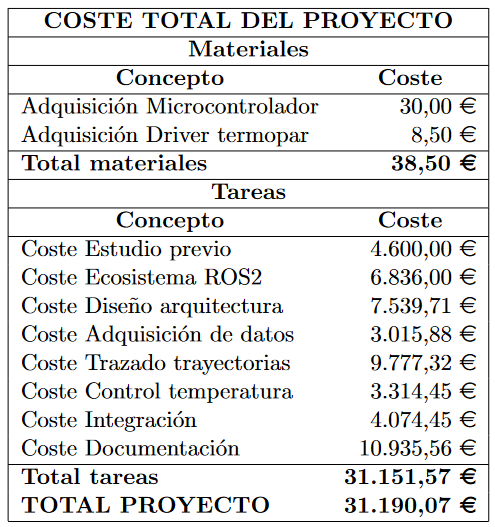
\includegraphics[scale=0.35]{figuras/coste_total_tabla.png}
    \caption{Coste total del proyecto}
    \label{tab:coste_total}
\end{table}

La tabla \ref{tab:horas_empleadas} muestra las horas dedicadas a la consecución del proyecto. Se asume un promedio de 4 horas dedicadas cada día. Dividiendo el total de horas de proyecto se obtienen los días proyectados en el calendario, que equivalen aproximadamente a 37 semanas. Es decir a lo planificado por la Figura \ref{fig:gantt}

\begin{table}[h!]
    \centering
    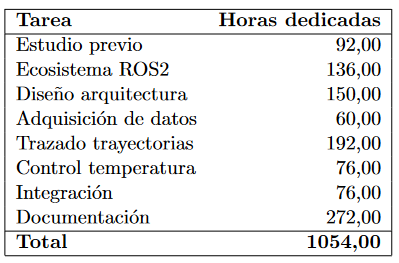
\includegraphics[scale=0.5]{figuras/horas_empleadas_tabla.png}
    \caption{Horas empleadas en el proyecto}
    \label{tab:horas_empleadas}
\end{table}
